\section{Periodic Boundary Conditions}
To simulate infinitely periodic structures periodic boundary conditions can be used. The Bloch-Theorem applied to the electromagnetic field states that for structures beeing periodic in two dimensions only a single unit-cell must be modelled, since 
\begin{equation}
\mathbf{E}(t,\mathbf{r}+\mathbf{R}_{nm}) =  \mathbf{E}\left(t\pm\frac{|\mathbf{r}-\mathbf{R}_{mn}|}{c}, \mathbf{r}\right) \exp(-\imag \mathbf{R}_{mn}\cdot \mathbf{k})
\end{equation}
if $\mathbf{R}_{mn}$ is a vector connecting the simulated unit-cell with its neighbour $m$ times the unit-cell length $L_x$ in $\unitv{x}$-direction and $n$ times the unit-cell length $L_y$ in $\unitv{y}$-direction:
\begin{equation}
\mathbf{R}_{mn} = m L_x \unitv{x} + n L_y \unitv{y},\quad m,n\in \mathbb{Z}
\end{equation}
and $k$ is the Bloch-wavevector. From now on we will assume periodic boundary conditions in both, $x$ and $y$ coordinates. If a periodic structure is illuminated by an obliquely incident plane wave with wavevector $\mathbf{k}^\mathrm{inc}$, the phase of the wave differes by $\mathbf{k}^\mathrm{inc}\cdot (\mathbf{r}+\mathbf{R}_{mn})$ between the simulated unit-cell and the cell indexed by $m$ and $n$. Lets consider the case:
\begin{equation}
\mathbf{k}^\mathrm{inc} = k^\mathrm{inc}\left(\sin\theta\cos\phi, \sin\theta\sin\phi,\cos\theta\right)^T
\end{equation}
where $\theta$ and $\phi$ specify the polar and azimuth angle of the incident wavevector which has modulus $|\mathbf{k}^\mathrm{inc}|=k^\mathrm{inc}$. For a monocromatic plane wave of frequency $\omega$ we can discriminate fields where either the electric or the magnetic field does not possess a component in $\unitv{z}$-direction which we will refer to by the notation $\mathbf{E}^\mathrm{TE_z}$ and $\mathbf{H}^\mathrm{TM_z}$. The direction $\bm{\xi}$ of the transverse component of those fields can be described by another angle $\gamma$:
\begin{equation}
\bm{\xi} = \left(\cos\gamma, \sin\gamma, 0 \right)^T.
\end{equation}
We can therefore write a $\mathrm{TE}_z$ incident field as
\begin{equation}
\mathbf{E}^\mathrm{TE_z} = E_0 \exp(-\imag \omega t)
\left(
\begin{array}{c}
\cos\gamma \\ \sin\gamma \\ 0
\end{array}\right)
\exp\big(\imag k^\mathrm{inc} (\sin\theta\cos\phi\; x + \sin\theta\sin\phi\; y + \cos\theta\; z\big)
\end{equation}
\begin{figure}
\centering
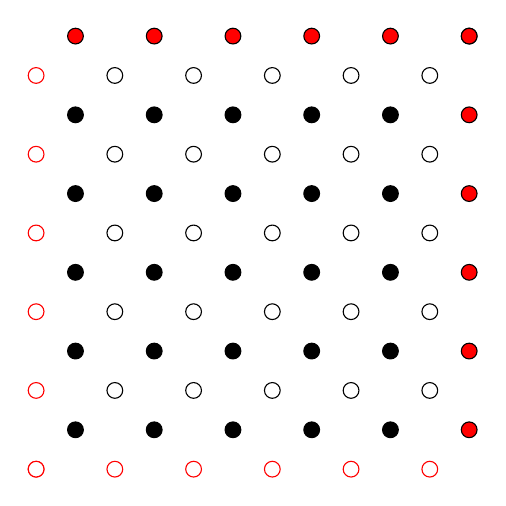
\begin{tikzpicture}
\foreach \i in {0,...,5}{
	\draw[red,fill=white] (\i+0.5,0.5) circle[radius=0.1cm]; 
	\draw[red,fill=white] (0.5,\i+0.5) circle[radius=0.1cm]; 
	\draw[fill=red] (6,\i+1) circle[radius=0.1cm]; 
	\draw[fill=red] (\i+1,6) circle[radius=0.1cm]; 
}
\foreach \x in {1,...,5}{
\foreach \y in {1,...,5}{
	\draw[fill=black] (\x,\y) circle[radius=0.1cm]; 
	\draw[fill=white] (\x+0.5,\y+0.5) circle[radius=0.1cm]; 
	
}}
\end{tikzpicture}
\caption{Indication of the nodes where the voltages 
(\protect\tikz\protect\draw[black,fill=black] (0,0) circle (.1cm);) and currents
(\protect\tikz\protect\draw[black,fill=white] (0,0) circle (.1cm);) are defined. The update of currents/voltages at the border of the grid is a priori not possible, since there are values missing at the nodes as indicated by symbols drawn in red. }
\end{figure}

However, due to the periodic boundary conditions we can obtain the missing voltages and currents as:
\begin{align}
u(N_x,n_y,n_z) &= u(0,n_y,n_z) \exp(\imag k_x L_x)\\
i(-1,n_y,n_z) &= i(N_x,n_y,n_z) \exp(-\imag k_y L_y)
\end{align}

The update equation for $u_x$ therefore becomes:
\begin{align}
\nonumber
&& u_x^{n_t+1}(0,n_y,n_z) = \mathrm{VV}_x(0,n_y,n_z)u^{n_t}(0,n_y,n_z)+ \\ 
&&\mathrm{VI}_x(0,n_y,n_z)\big[
i_z^{\tilde{n}_t}(0,\tilde{n}_y,\tilde{n}_z)-i_z^{\tilde{n}_t}(0,\tilde{n}_y-1,\tilde{n}_z)+
i_y^{\tilde{n}_t}(0,\tilde{n}_y,\tilde{n}_z-1)-i_z^{\tilde{n}_t}(0,\tilde{n}_y,\tilde{n}_z)
\big].
\end{align}

$\mathrm{VV}$ and $\mathrm{VI}$ indicate the voltage-voltage and voltage-current update-coefficients. Since the updating process for boundary values of $u/i$ will be treated in an engine extension of openEMS, we will set the coefficient $\mathrm{VV}/\mathrm{VI}$ to $1/0$ at the minimum $x$ and $y$-coordinate. 

For the voltage/current updates on the PBC plane at $x=0$/$x=x_\mathrm{max}$ we need currents/voltages which must be fetched from the opposite side of the grid meaning:
\begin{align}
&& I[0] &= I[\mathrm{max}] \exp(-\imag kL),\\
&& U[\mathrm{max}] &= U[0] \exp(\imag kL).
\end{align}
Splitted into real and imaginary parts this means:
\begin{align}
&&\Re{I[0]} &= \cos(kL)\Re{I[\mathrm{max}]} +\sin(kL) \Im{I[\mathrm{max}]},\\
&&\Im{I[0]} &= \cos(kL)\Im{I[\mathrm{max}]} -\sin(kL) \Re{I[\mathrm{max}]},\\
&&\Re{U[\mathrm{max}]} &= \cos(kL)\Re{U[0]} - \sin(kL) \Im{U[0]},\\
&&\Im{U[\mathrm{max}]} &= \cos(kL)\Im{U[0]} + \sin(kL) \Re{U[0]}.
\end{align}
